%**************************************************************************
%* SpringSim 2019 Author Kit
%*
%* Word Processing System: TeXnicCenter and MiKTeX
%*
%**************************************************************************
\documentclass{scspaperproc}

\usepackage{latexsym}
\usepackage{graphicx}
\usepackage{mathptmx}

%
%****************************************************************************
% AUTHOR: You may want to use some of these packages. (Optional)
%\usepackage{amsmath}
%\usepackage{amsfonts}
%\usepackage{amssymb}
%\usepackage{amsbsy}
%\usepackage{amsthm}
%****************************************************************************


%
%****************************************************************************
% AUTHOR: If you do not wish to use hyperlinks, then just comment
% out the hyperref usepackage commands below.

%% This version of the command is used if you use pdflatex. In this case you
%% cannot use ps or eps files for graphics, but pdf, jpeg, png etc are fine.

\usepackage[pdftex,colorlinks=true,urlcolor=blue,citecolor=black,anchorcolor=black,linkcolor=black]{hyperref}

%% The next versions of the hyperref command are used if you adopt the
%% outdated latex-dvips-ps2pdf route in generating your pdf file. In
%% this case you can use ps or eps files for graphics, but not pdf, jpeg, png etc.
%% However, the final pdf file should embed all fonts required which means that you have to use file
%% formats which can embed fonts. Please note that the final PDF file will not be generated on your computer!
%% If you are using WinEdt or PCTeX, then use the following. If you are using
%% Y&Y TeX then replace "dvips" with "dvipsone"

%% \usepackage[dvips,colorlinks=true,urlcolor=blue,citecolor=black,%
%% anchorcolor=black,linkcolor=black]{hyperref}

%% The use of the long citation format (e.g. "Brown and Edwards (1993)" rather than "[5]") and at the same
%% time using the hyperref package can lead to hard to trace bugs in case the citation is broken accross the
%% line (usually this will mark the entire paragraph as a hyperlink (clickable) which is easily noticeable and fixed
%% if using colorlinks, but not if the color is black -- as it is now). Worse yet, if a citation spans page boundary,
%% LaTeX compilation can fail, with an obscure error message. Since this depends a lot on the flow of the text
%% and wording, these bugs come and go and can be extremely hard for a beginner to trace. The error
%% message can look like this:
%%
%%    ! pdfTeX error (ext4): \pdfendlink ended up in different nesting level than \pdfstartlink.
%%    \AtBegShi@Output ...ipout \box \AtBeginShipoutBox 
%%    \fi \fi 
%%    l.174 
%%    ! ==> Fatal error occurred, no output PDF file produced!
%%
%% and can be universally fixed by putting an \mbox{} around the citation in question (in this case, at line 174)
%% and maybe adapting the wording a little bit to improve the paragraph typesetting, which is perhaps not
%% immediately obvious.
%****************************************************************************

%
%****************************************************************************
%*
%* AUTHOR: YOUR CALL!  Document-specific macros can come here.
%*
%****************************************************************************

\usepackage{float}
\usepackage{subcaption}
\usepackage{minted}
\usepackage{verbatim}

%#########################################################
%*
%*  The Document.
%*
\begin{document}

%***************************************************************************
% AUTHOR: AUTHOR NAMES GO HERE
% FORMAT AUTHORS NAMES Like: Author1, Author2 and Author3 (last names)
%
%		You need to change the author listing below!
%               Please list ALL authors using last name only, separate by a comma except
%               for the last author, separate with "and"
%
\SCSpagesetup{Thaler, Siebers and Altenkirch}

% AUTHOR: Uncomment ONE of these correct conference names.
%\def\SCSconferenceacro{SpringSim}
\def\SCSconferenceacro{SummerSim}
%\def\SCSconferenceacro{AutumnSim}
%\def\SCSconferenceacro{PowerPlantSim}

% AUTHOR: Set the correct year of the conference.
\def\SCSpublicationyear{2019}

% AUTHOR: Set the correct month and dates; the dates are separated by a single minus sign
% with no spaces and no leading zeros, the month is a full name (e.g. April) with the first letter
% capitalized. For example, "April 8-13".
\def\SCSconferencedates{July 22-July 24}

% AUTHOR: Set the correct venue in the form "City, State, Country", for example "Los Angeles, CA, USA".
\def\SCSconferencevenue{Berlin, Germany}

% AUTHOR: Uncomment ONE of the track/symposium names where you are going to submit. Please, do NOT change.
% In case your symposium is not on this list, please DO contact your symposium chair.
\def\SCSsymposiumacro{ANSS} % Annual Simulation Symposium
%\def\SCSsymposiumacro{CNS} % Communications and Networking Simulation Symposium
%\def\SCSsymposiumacro{HPC} % High Performance Computing Symposium
%\def\SCSsymposiumacro{TMS/DEVS} % Symposium on Theory of Modeling and Simulation
%\def\SCSsymposiumacro{ADS} % Agent-Directed Simulation
%\def\SCSsymposiumacro{MSCIAAS} % Modeling and Simulation of Complexity in Intelligent, Adaptive and Autonomous Systems
%\def\SCSsymposiumacro{MSM} % Modeling and Simulation in Medicine
%\def\SCSsymposiumacro{Mod4Sim} % Model-driven Approaches for Simulation Engineering Symposium
%\def\SCSsymposiumacro{Tutorial} % Tutorial Track
%\def\SCSsymposiumacro{WIP} % WIP Track
%\def\SCSsymposiumacro{Poster/Colloquium} % Poster Session and Student Colloquium
%\def\SCSsymposiumacro{MobileApp} % Student M\&S Mobile App Competition
%\def\SCSsymposiumacro{SPECTS} % Symposium on Performance Evaluation of Computer and Telecommunication Systems
%\def\SCSsymposiumacro{SCSC} % Summer Computer Simulation Conference
%\def\SCSsymposiumacro{ICBGM} % International Conference on Bond-Graph Modeling
%\def\SCSsymposiumacro{Fossil} % Fossil Power Track
%\def\SCSsymposiumacro{Nuclear} % Nuclear Agent Power Track

% AUTHOR: Enter the title, all letters in upper case

\newminted[HaskellCode]{haskell}{fontsize=\footnotesize}

% Title portion. Note the short title for running heads
\title{Hands Off My Property!}
%\subtitle{The Potential Of Property-Based Testing In Agent-Based Simulation}

% AUTHOR: Enter the authors of the article, see end of the example document for further examples
\author{
\\%To level with the author block on the right.
Jonathan Thaler \\ 
Peer Olaf Siebers \\ [12pt] 
School Of Computer Science \\
University of Nottingham \\
7301 Wollaton Rd \\
Nottingham, United Kingdom \\
\{jonathan.thaler,peer-olaf.siebers\}@nottingham.ac.uk\\
}



\maketitle

\section*{Abstract}
%- there are two possible sub-tracks for it: Agent-based Modeling and Simulation (ABMS) or Verification and Validation of Computer Simulation Models (V&V).

This paper presents a new and complementary approach to unit-testing the implementation of agent-based simulations, called property-based testing which allows to test specifications and laws of the implementation directly in code which is then tested using \textit{automated} test-data generation. We present two different models as case-studies in which we will show how to apply property-based testing to exploratory and explanatory agent-based models and what its limits are.

\textbf{Keywords:} Agent-Based Simulation, Validation \& Verification, Property-Based Testing.

\maketitle

\section{Introduction}
There exists a large number of simulation packages which allow the convenient creation of System Dynamics simulations by straight-forward visual diagram creation. One simply creates stocks and flows, connects them, specifies the flow-rates and initial parameters and then runs the model. An example for such a visual diagram creation in the simulation package AnyLogic can be seen in Figure \ref{fig:sir_stockflow_diagram}.

\begin{figure}
	\centering
	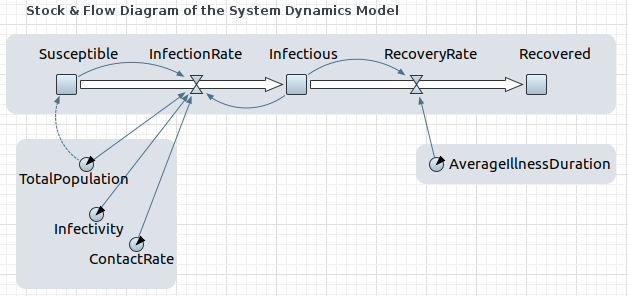
\includegraphics[width=.5\textwidth, angle=0]{./fig/SIR_SD_STOCKFLOW_DIAGRAMM.png}
	\caption{Visual System Dynamics Diagram of the SIR model in AnyLogic Personal Learning Edition 8.3.1.}
	\label{fig:sir_stockflow_diagram}
\end{figure}

Still, implementing System Dynamics directly in code is not as straight forward and involves numerical integration which can be quite tricky to get right. Thus, the aim of this paper is to look into how System Dynamics models can be implemented in code correctly without the use of a simulation package. We use the well known SIR model \cite{kermack_contribution_1927} from epidemiology to demonstrate our approach.

Our language of choice is Haskell because it emphasises a declarative programming style in which one describes \textit{what} instead of \textit{how} to compute. Further it allows to rule out interference with non-deterministic influences or side-effects already at compile-time. This is of fundamental importance for System Dynamics because it behaves completely deterministic and involves no stochastics or non-determinism whatsoever. Also, we make use of Functional Reactive Programming which allows to express continuous-time systems in a functional way. 

We show that by this approach we can arrive at correct-by-construction implementations of System Dynamic models. This means that the correctness of the code is obvious because we have closed the gap between the model specification and its implementation. Thus, the contribution of the paper is the demonstration of how to implement correct-by-construction System Dynamics simulations using Haskell and Functional Reactive Programming.

\section{Related Workd}
\label{sec:related}

% related works
% read all the papers peer has sent me
% https://www.atlassian.com/continuous-delivery/different-types-of-software-testing
%% TDD in ABS
Research on TDD of ABS is quite new and thus there exist relative few publications. The work \cite{collier_test-driven_2013} is the first to discusses how to apply the TDD approach to ABS, using unit-testing to verify the correctness of the implementation up to a certain level. They show how to implement unit-tests within the RePast Framework \cite{north_complex_2013} and make the important point that such a software need to be designed to be sufficiently modular otherwise testing becomes too cumbersome and involves too many parts. The paper \cite{asta_investigation_2014} discusses a similar approach to DES in the AnyLogic software toolkit. 

The paper \cite{onggo_test-driven_2016} proposes Test Driven Simulation Modelling (TDSM) which combines techniques from TDD to simulation modelling. The authors present a case study for maritime search-operations where they employ ABS. They emphasise that simulation modelling is an iterative process, where changes are made to existing parts, making a TDD approach to simulation modelling a good match. They present how to validate their model against analytical solutions from theory using unit-tests by running the whole simulation within a unit-test and then perform a statistical comparison against a formal specification. This approach will become of importance later on in our SIR case study.

The paper \cite{brambilla_property-driven_2012} propose property-driven design of robot swarms. They propose a top-down approach by specifying properties a swarm of robots should have from which a prescriptive model is created, which properties are verified using model checking. Then a simulation is implemented following this prescriptive and verified model after then the physical robots are implemented. The authors identify the main difficulty of implementing such a system that the engineer must \textit{"think at the collective-level, but develop at the individual-level}. It is arguably true that this also applies to implementing agent-based models and simulations where the same collective-individual separation exists from which emergent system behaviour of simulations emerges - this is the very foundation of the ABS methodology.

The paper \cite{gurcan_generic_2013} gives an in-depth and detailed overview over verification, validation and testing of agent-based models and simulations and proposes a generic framework for it. The authors present a generic UML class model for their framework which they then implement in the two ABS frameworks RePast and MASON. Both of them are implemented in Java and the authors provide a detailed description how their generic testing framework architecture works and how it utilises JUnit to run automated tests. To demonstrate their framework they provide also a case study of an agent-base simulation of synaptic connectivity where they provide an in-depth explanation of their levels of test together with code.

The review of the literature in the field gives the impression, that most research focuses on high-level validation and does not deal too much with verification on a technical, code-base level.

%% TDD in MAS
Although the work on TDD is scarce in ABS, there exists quite some research on applying TDD and unit-testing to multi-agent systems (MAS). Although MAS is a different discipline than ABS, the latter one has derived many technical concepts from the former one thus testing concepts applied to MAS might also be applicable to ABS. The paper \cite{nguyen_testing_2011} is a survey of testing in MAS. It distinguishes between unit tests which tests units that make up an agent, agent tests which test the combined functionality of units that make up an agent, integration tests which test the interaction of agents within an environment and observe emergent behaviour, system test which test the MAS as a system running at the target environment and acceptance test in which stakeholders verify that the software meets their goal. Although not all ABS simulations need acceptance and system tests, still this classification gives a good direction and can be directly transferred to ABS.  %Further the paper enumerates existing research and shows that some research is working on generating automated test input for agent level tests. 

%The paper \cite{tiryaki_sunit:_2007} discusses Test Driven Development in MAS and puts much emphasis on proposing agile processes to develop MAS software to handle complexity and continuously changing nature of requirements. The authors develop the SUNIT testing framework to implement unit-testing in an MAS environment.

\section{Property-Based Testing}
\label{sec:proptesting}

Property-based testing allows to formulate \textit{functional specifications} in code which then a property-based testing library tries to falsify by \textit{automatically} generating test-data, covering as many cases as possible. When a case is found for which the property fails, the library then reduces the test-data to its simplest form for which the test still fails e.g. shrinking a list to a smaller size. It is clear to see that this kind of testing is especially suited to ABS, because we can formulate specifications, meaning we describe \textit{what} to test instead of \textit{how} to test. Also the deductive nature of falsification in property-based testing suits very well the constructive and exploratory nature of ABS. Further, the automatic test-generation can make testing of large scenarios in ABS, which is almost always stochastic by nature, feasible as it does not require the programmer to specify all test-cases by hand, as is required in traditional unit-tests.

Property-based testing was invented by the authors of \cite{claessen_quickcheck_2000,claessen_testing_2002} in which they present the QuickCheck library in Haskell, which tries to falsify the specifications by \textit{randomly} sampling the space. We argue, that the stochastic sampling nature of this approach is particularly well suited to ABS, because it is itself almost always driven by stochastic events and randomness in the agents behaviour, thus this correlation should make it straight-forward to map ABS to property-testing. A challenge when using QuickCheck is to write \textit{custom} test-data generators for agents and the environment, which cover the space sufficiently enough to not miss out on important test-cases. According to the authors of QuickCheck \textit{"The major limitation is that there is no measurement of test coverage."} \cite{claessen_quickcheck_2000}. QuickCheck provides help to report the distribution of test-cases but still it could be the case that simple test-cases which would fail are never tested because of the stochastic nature of QuickCheck.

To give a rough idea on how property-based testing works in Haskell, we give a few examples of properties on lists, which are directly expressed as functions in Haskell. Such a function has to return a \textit{Bool}, which indicates \textit{True} in case the test succeeds or \textit{False} if not and can take input arguments which data is automatically generated by QuickCheck. Note that the first line of each function defines its name, its inputs (\textit{[Int]} is a list of integers) and the output which is the last type (\textit{Bool}). Note that the \textit{(++)} operator concatenates two lists, \textit{reverse} simply reverses a list.

\begin{HaskellCode}
-- concatenation operator (++) is associative
append_associative :: [Int] -> [Int] -> [Int] -> Bool
append_associative xs ys zs = (xs ++ ys) ++ zs == xs ++ (ys ++ zs)

-- reverse is distributive over concatenation (++)
-- xs and ys need to be swapped on the right-hand side!
reverse_distributive :: [Int] -> [Int] -> Bool
reverse_distributive xs ys = reverse (xs ++ ys) == reverse ys ++ reverse xs

-- the reverse of a reversed list is the original list
reverse_reverse :: [Int] -> Bool
reverse_reverse xs = reverse (reverse xs) == xs
\end{HaskellCode}

% POTENTIAL FOR SHORTENING
As a remedy for the potential sampling difficulties of QuickCheck, there exists also a deterministic property-testing library called SmallCheck \cite{runciman_smallcheck_2008}, which instead of randomly sampling the test-space, enumerates test-cases exhaustively up to some depth. It is based on two observations, derived from model-checking, that (1) \textit{"If a program fails to meet its specification in some cases, it almost always fails in some simple case"} and (2) \textit{"If a program does not fail in any simple case, it hardly ever fails in any case} \cite{runciman_smallcheck_2008}. This non-stochastic approach to property-based testing might be a complementary addition in some cases, where the tests are of non-stochastic nature with a search-space which is too large to implement manually by unit-tests but is relatively easy and small enough to enumerate exhaustively. The main difficulty and weakness of using SmallCheck is to reduce the dimensionality of the test-case depth search to prevent combinatorial explosion, which would lead to an exponential number of cases. Thus, one can see QuickCheck and SmallCheck as complementary instead of in opposition to each other.
% POTENTIAL FOR SHORTENING
Note that in this paper we only use QuickCheck due to the match of ABS stochastic nature and the random test generation. Also note that we regard property-based testing as \textit{complementary} to unit-tests and not in opposition - we see it as an addition in the TDD process of developing an ABS.

\section{Verifying ABS implementations}
\label{sec:verifyingABS}

in ABS depending on which level we are, property-based testing means different things and does not necessarily involve QuickCheck and can also be technically implemented as unit-tests

Generally we need to distinguish between two types of testing/verification: 1. testing/verification of models for which we have real-world data or an analytical solution which can act as a ground-truth - examples for such models are the SIR model, stock-market simulations, social simulations of all kind and 2. testing/verification of models which are just exploratory and which are only be inspired by real-world phenomena - examples for such models are Epsteins Sugarscape and Agent\_Zero.

So the baseline is that either one has an analytical model as the foundation of an agent-based model or one does not. In the former case, e.g. the SIR model, one can very easily validate the dynamics generated by the simulation to the one generated by the analytical solution through System Dynamics. In the latter case one has basically no idea or description of the emergent behaviour of the system prior to its execution e.g. SugarScape. In this case it is important to have some hypothesis about the emergent property / dynamics. The question is how verification / validation works in this setting as there is no formal description of the expected behaviour: we don't have a ground-truth against which we can compare our simulation dynamics.

\subsection{Black-Box Verification}
In black-box Verification one generally feeds input and compares it to expected output. In the case of ABS we have the following examples of black-box test:
\begin{enumerate}
	\item Isolated Agent Behaviour - test isolated agent behaviour under given inputs using and property-based testing.
	\item Interacting Agent Behaviour - test if interaction between agents are correct .
	\item Simulation Dynamics - compare emergent dynamics of the ABS as a whole under given inputs to an analytical solution or real-world dynamics in case there exists some using statistical tests.
	\item Hypotheses- test whether hypotheses are valid or invalid using and property-based testing. % TODO: how can we formulate hypotheses in unit- and/or property-based tests?
\end{enumerate}

%- testing of the final dynamics: how close do they match the analytical solution
%- can we express model properties in tests e.g. quickcheck?
%- property-testing shines here
%- isolated tests: how easy can we test parts of an agent / simulation?

Using black-box verification and property-based testing we can apply for the following use cases for testing ABS in FRP:

\subsection{White-Box Verification}
White-Box verification is necessary when we need to reason about properties like \textit{forever}, \textit{never}, which cannot be guaranteed from black-box tests. Additional help can be coverage tests with which we can show that all code paths have been covered in our tests.

TODO: List of Common Bugs and Programming Practices to avoid them \cite{vipindeep_list_2005}

We have discussed in this section \textit{how} to approach an ABS implementation from a pure functional perspective using Haskell where we have also briefly touched on \textit{why} one should do so and what the benefits and drawbacks are. In the next two sections we will expand on the \textit{why} by presenting two case-studies which show the benefits of using Haskell in regards of testing and increasing the confidence in the correctness of the implementation.

\section{Case Study I: SIR}
\label{sec:case_SIR}

As first use-case we discuss property-based testing for the agent-based SIR model. It is a very well studied and understood compartment model from epidemiology \cite{kermack_contribution_1927} which allows to simulate the dynamics of an infectious disease like influenza, tuberculosis, chicken pox, rubella and measles spreading through a population. We implemented an agent-based version of this model \footnote{The code is freely accessible from \url{https://github.com/thalerjonathan/phd/tree/master/public/propabs/sir}}, which is inspired by \cite{macal_agent-based_2010}.

In this model, people in a population of size $N$ can be in either one of three states \textit{Susceptible}, \textit{Infected} or \textit{Recovered} at a particular time, where it is assumed that initially there is at least one infected person in the population. People interact \textit{on average} with a given rate of $\beta$ other people per time-unit and become infected with a given probability $\gamma$ when interacting with an infected person. When infected, a person recovers \textit{on average} after $\delta$ time-units and is then immune to further infections. An interaction between infected persons does not lead to re-infection, thus these interactions are ignored in this model. Due to the models origins in System Dynamics (SD) \cite{porter_industrial_1962}, there exists a top-down formalisation in SD with the following equations:

\begin{equation}
\frac{\mathrm d S}{\mathrm d t} = -infectionRate \\ 
\frac{\mathrm d I}{\mathrm d t} = infectionRate - recoveryRate \\ 
\frac{\mathrm d R}{\mathrm d t} = recoveryRate 
\end{equation}

\begin{equation}
infectionRate = \frac{I \beta S \gamma}{N} \\
recoveryRate = \frac{I}{\delta} 
\end{equation}

\subsection{Deriving a property}
Our goal is to derive a property which connects the agent-based implementation to the SD equations. The foundation are both the infection- and recovery-rate where the infection-rate determines how many \textit{Susceptible} agents per time-unit become \textit{Infected} and the recovery-rate determines how many \textit{Infected} agents per time-unit become \textit{Recovered}. Lets look at the pseudo-code of the susceptible agent behaviour, which is key for the infection-rate:

\begin{algorithm}
generate on average $\beta$ make-contact events per time-unit\; 
\If{make-contact event}{
  select random agent \textit{randA} from population\; 
  \If{agent randA infected}{
    become infected with probability $\gamma$\; 
  }  
}
\caption{Susceptible behaviour}
\end{algorithm}

Per time-unit, a susceptible agent makes \textit{on average} contact with $\beta$ other agents where in the case of a contact with an infected agent the susceptible agent becomes infected with a given probability $\gamma$. In this description there is another probability hidden, which is the probability of making contact with an infected agent which is simply the ratio of number of infected agents to number non-infected agents. We can now derive the formula for the probability of a \textit{Susceptible} agent to become infected: $\beta * \gamma * \frac{number of infected}{number of non-infected}$. When we look at the formula we can see that it is conceptually the same representation of the \textit{infection-rate} of the SD specification as shown above - except that it only considers a single \textit{Susceptible} agent instead of the aggregate of \textit{S} susceptible agents. We have now a property we can check using a property-based test.

\subsection{Constructing the property-based test}
Having a property (law), we want now to construct a property-based test for it. The formula is invariant under random population mixes and thus should hold for varying agent populations where the mix of \textit{Susceptible, Infected and Recovered} agents is random - thus we use QuickCheck to generate the population randomly, the property must still hold.

Obviously we need to pay attention to the fact that we are dealing with a stochastic system thus we can only talk about averages and thus it does not suffice to only run a single agent but we are repeating this for e.g. 10.000 \textit{Susceptible} agents (all with different random-number seeds). 

To check whether this test has passed we compare the required amount of agents which on average should become infected using the above formula to the one from our tests (simply count the agents which got infected and divide by N) and if the value lies within some small $\epsilon$ then we accept the test as passed. Now we can construct the following property-based test as shown in Algorithm \ref{alg:prop_test_infectionrate}.

\begin{algorithm}
\SetKwInOut{Input}{input}\SetKwInOut{Output}{output}
\Input{List \textit{randAs} of random agent-population generated by QuickCheck}
populationCount     = length \textit{randAs}\;
infectedCount       = count \textit{Infected} in \textit{randAs}\;
infectionRate       = infectivity * contactRate * (infectedCount / populationCount)\;

susceptibles = 10000\;
countInfected = 0\;
\For{$i\leftarrow 1$ \KwTo $susceptibles$}{
  create \textit{Susceptible} agent sa\;
  run agent sa for 1.0 time-unit, with list \textit{randAs} as input\;
  \If{agent sa became \textit{Infected} }{
	countInfected = countInfected + 1\;
  }
}

actualInfectionRate = countInfected / susceptibles\;
$\epsilon$ = 0.1\;
\eIf{abs (actualInfectionRate - infectionRate) $\leq \epsilon$}{
  PASS\;
} {
  FAIL\;
}
\caption{Property-based test for infection-rate.}
\end{algorithm}
\label{alg:prop_test_infectionrate}

When running, QuickCheck generates 100 random test-cases by randomly generating 100 different \textit{randAs} inputs to the test. All have to pass for the whole property-test to pass, which should be the case with an $\epsilon = 0.1$. 

This is the very power which property-based testing is offering us: we directly express the specification of the original SD model in a test of our agent-based implementation and let QuickCheck generate random test cases for us. This closely ties our implementation to the original specification and "proves" that it is actually a valid implementation.

%\subsection{Infected Behaviour}
%An infected agent will \textit{always} recover after some finite time, which is \textit{on average} after $\delta$ time-units. Note that this property involves stochastics too, so to test this property we run a large number of infected agents e.g. $N = 10.000$ (all with different random-number seeds) until they recover, record the time of each agents recovery and then average over all recovery times. To check whether this test has passed we compare the average recovery times to $\delta$ and if they lie within some small $\epsilon$ then we accept the test as passed (note again that we could use a t-test for better stochastic robustness but this is not the point of this paper).
%
%TODO: clearly state the property we test
%
%TODO: produce some pseudo-code of how the property-test conceptually works
%
%in the infected agent test we check if the average duration is as specified. does this resemble the recovery rate? or in other words: can we somehow test the recovery rate?
%durationsAvg = sum durations / fromIntegral (length durations)
%
%We use property-testing with QuickCheck in this case as well to generate the set of other agents as input for the infected agents. Strictly speaking this would not be necessary as an infected agent never makes contact with other agents and simply ignores them - we could as well just feed in an empty list. We opted for using QuickCheck for the following reasons:
%
%\begin{itemize}
%	\item We wanted to stick to the interface specification of the agent-implementation as close as possible which asks to pass the states of all agents as input.
%	\item We shouldn't make any assumptions about the actual implementation and if it REALLY ignores the other agents, so we strictly stick to the interface which requires us to input the states of all the other agents.
%	\item The set of other agents is ignored when determining whether the test has failed or not which indicates by construction that the behaviour of an infected agent does not depend on other agents.
%	\item We are not just running a single replication over 10.000 agents but 100 of them which should give black-box verification more strength.
%\end{itemize}
%
%\subsection{Recovered Behaviour}
%A recovered agent will stay recovered \textit{forever}. Obviously we cannot write a property-based test that truly verifies that because it had to run in fact \textit{forever}. In this case we need to resort to white-box verification and look directly at the code and reason whether this property holds true.

\section{Case Study II: SugarScape}
\label{sec:case_sug}
We now look at how property-based testing can be made of use in the \textit{exploratory} Sugarscape model \cite{epstein_growing_1996}. It was one of the first models in ABS, with the aim to \textit{grow} an artificial society by simulation and connect observations in their simulation to phenomenon observed in real-world societies. In this model a population of agents move around in a discrete 2D environment, where sugar grows, and interact with each other and the environment in many different ways. The main features of this model are (amongst others): searching, harvesting and consuming of resources, wealth and age distributions, population dynamics under sexual reproduction, cultural processes and transmission, combat and assimilation, bilateral decentralized trading (bartering) between agents with endogenous demand and supply, disease processes transmission and immunology. For our research we undertook a \textit{full and validated} implementation of the Sugarscape model \footnote{The code can be accessed freely from \url{https://github.com/thalerjonathan/haskell-sugarscape}}. We validated of our implementation against the book \cite{epstein_growing_1996} and a NetLogo implementation \cite{weaver_replicating_2009} \footnote{\url{https://www2.le.ac.uk/departments/interdisciplinary-science/research/replicating-sugarscape}} during which we also implemented property tests. Due to lack of space we added a discussion of the validation process as an Appendix \ref{app:validation}.

Whereas in the explanatory SIR case-study we had an analytical solution, inspired by the SD origins of the model, the fundamental difference in the exploratory Sugarscape model is that no such analytical solutions exist. This raises the question, which properties we can actually test in such a model - we propose the following:

\begin{itemize}
	\item Environment behaviour - the Sugarscape environment has its own behaviour which boils down to regrowing of resources. The correct working can be tested using property-tests by generating random environments and checking laws governing the regrowth.
	
	\item Agent behaviour - obviously full agent behaviour could be tested with property-tests, using randomly generated agents (with random values in their properties). It turned out to be quite difficult to derive properties for full agent behaviour, thus in this paper we restricted ourselves to test parts of agent behaviour and also left out testing of agent interactions.

	\item Emergent behaviour - although we don't have analytical descriptions of properties of our model in the case of Sugarscape, there still exist informal descriptions and more formal hypotheses about emergent properties. Property-testing can be used to check them and if proved to be valid can be seen as regression tests.
\end{itemize}

\subsection{Environment behaviour}
The environment in the Sugarscape model has some very simple behaviour: each site has a sugar level and when harvested by an agent, it regrows back to the full level over time. Depending on the configuration of the model it either grows back immediately within 1 tick or over multiple ticks. We can construct simple property-tests for these behaviours. In the case the sugar grows back immediately, we let QuickCheck generate a random environment and then run the environment behaviour for 1 tick and then check the property that all sites have to be back to their maximum sugar level. In the case of regrow over multiple ticks, we also use QuickCheck to generate a random environment but additionally a random \textit{positive} rate (which is a floating point number) which we then use to calculate the number of ticks until full regrowth. After running the random environment for the given number of ticks all sites have to be back to full sugar level - see Algorithm \ref{alg:prop_test_rateregwroth} for this case.

Note that QuickCheck initially doesn't know how to generate a random environment because each site consists of a custom data-structure for which QuickCheck is not able to generate random instances by default. This problem is solved by writing a custom data-generator, for which existing QuickCheck functions can be used e.g. picking the current sugar level of a site from a random range.

\begin{algorithm}
\SetKwInOut{Input}{input}\SetKwInOut{Output}{output}
\Input{Random environment \textit{env} generated by QuickCheck}
\Input{Random regrowth rate \textit{randRate} generated by QuickCheck}
maxTicks = maxSugarCapacityOnSites / randRate\;
env' = runEnvironmentTicks maxTicks env\;
sites = getEnvironmentSites env'\;

\eIf{all sites maxSugarLevel}{
  PASS\;
} {
  FAIL\;
}
\caption{Property-based test for rate-based regrow of sugar on all sites.}
\label{alg:prop_test_rateregwroth}
\end{algorithm}

The Sugarscape environment is a torus where the coordinates wrap around in both dimensions. To check whether the implementation of the wrapping calculation is correct we used both unit- and property-tests. With the unit-tests we carefully constructed all possible cases we could think of and came up with 13 test-cases. With the property-based test we simply defined a single test-case where we expressed the property, that after wrapping \textit{any} random coordinates supplied by QuickCheck, the wrapped coordinates have to be within bounds. See Algorithm \ref{alg:prop_test_wrapcoords}.

\begin{algorithm}
\SetKwInOut{Input}{input}\SetKwInOut{Output}{output}
\Input{Random 2D discrete coordinate \textit{randCoord} generated by QuickCheck}
(x, y) = wrapCoordinates randCoord\;

\eIf{(x $\geq$ 0 and x $\leq$ environmentDimX) and (y $\geq$ 0 and y $\leq$ environmentDimY)}{
  PASS\;
} {
  FAIL\;
}
\caption{Property-based test for wrap-coordinates functionality.}
\label{alg:prop_test_wrapcoords}
\end{algorithm}

\subsection{Agent behaviour}
We implemented a number of property-tests for agent functions which just cover a part of an agents behaviour: checks whether an agent has died of age or starved to death, the metabolism, immunisation step, check if an agent is a potential borrower or fertile, lookout, trading transactions. We provided custom data-generators for the agents and let QuickCheck generate the random data and us running the agent with the provided data, checking for the properties. 

As an example, provided in Algorithm \ref{alg:prop_test_agent}, we give the property-test of an agent dying of age, which happens when the agents age is greater or equal its maximum age. It might look trivial but property-based testing helps us here to clearly state the invariants (properties) and relieves us from constructing all possible edge-cases because we rely on QuickChecks abilities to cover them for us.

\begin{algorithm}
\SetKwInOut{Input}{input}\SetKwInOut{Output}{output}
\Input{Random agent \textit{ag} with random age generated by QuickCheck}
died = hasAgentDiedOfAge ag;\

\eIf{died == (age ag >= maxAge ag)} {
  PASS\;
} {
  FAIL\;
}
\caption{Property-based test for agent dying of age.}
\label{alg:prop_test_agent}
\end{algorithm}

\subsection{Emergent properties}
In the validation and verification process of our Sugarscape implementation we put informal descriptions and hypotheses about emergent properties from the Sugarscape book into formal property-tests. Examples for such hypotheses / informal descriptions of emergent properties are e.g. the carrying capacity becomes stable after 100 steps; when agents trade with each other, after 1,000 steps the standard deviation of trading prices is less than 0.05; when there are cultures, after 2,700 steps either one culture dominates the other or both are equally present.

The property we test for is whether \textit{the emergent property under test is stable under varying random-number seeds} or not. Put another way, we let QuickCheck generate random number streams and require that the tests all pass. Unfortunately, this revealed that this property doesn't hold for all hypotheses. The problem is that QuickCheck generates by default 100 test-cases for each property-test where all need to pass for the whole property-test to pass - this wasn't the case, where most of the 100 test-cases passed but unfortunately not all. Thus in this case a different approach is required: instead of requiring \textit{every} test to pass we require that \textit{most} tests pass, which can be achieved using a T-test with a confidence interval of e.g. 95\%. This means we won't use QuickCheck anymore and resort to a normal unit-test where we run the simulation 100 times with different random number streams each time and then performing a T-test with a 95\% confidence interval. Note that we are now technically speaking of a unit-test but conceptually it is still a property-test.

In Algorithm \ref{alg:prop_test_trading} we show a property-test for checking whether after 1,000 steps the standard deviation of trading prices is less than 0.05. The test passes if out of 100 runs a 95\% confidence interval is reached using a T-test.

\begin{algorithm}
maxTicks = 1000\;
replications = 100\;
stdAverage = 0.05\;
tradingPriceStdsList = empty list\;

\For{$i\leftarrow 1$ \KwTo replications}{
rng = new random number generator\;
simContext = initSimulation rng\;
out = runSimulation maxTicks simContext\;
tps = extractTradingPrices out\;
tpsStd = calculate standard deviation of tps\;
insert tpsStd into tradingPriceStdsList\;
}

tTestPass = perform 1-sided t-test comparing stdAverage with tradingPriceStdsList on a 0.95 interval\;

\eIf{tTestPass}{
  PASS\;
} {
  FAIL\;
}
\caption{Property-based test for trading prices.}
\label{alg:prop_test_trading}
\end{algorithm}

\chapter{Conclusions}
\label{chap:concl}

\section{Being Realistic}
It is of most importance to stress that we don't condemn the current state-of-the-art approach of object-oriented specification and implementation to ABS. The strength of object-oriented programming is surely that it can be seen as \textit{programming as modelling} and thus will be always an attractive approach to ABS. Also we are realists and know that there are more points to consider when selecting a set of methods for developing software for an ABS than robustness, verification and validation. Almost always the popularity of an existing language and which languages the implementer knows is the driving force behind which methods and languages to choose. This means that ABS will continue to be implemented in object-oriented programming languages and many perfectly well functioning models will be created by it in the future. Although they all suffer from the same issues mentioned in the introduction this doesn't matter as they are not of central importance to most of them.
Nonetheless we think our work is still essential and necessary as it may start a slow paradigm-shift and opens up the minds of the ABS community to a more functional and formal way of approaching and implementing agent-based models and simulations and recognizing the benefits one gets automatically from it by doing so.

\section{What we are not doing}
Because of this highly interdisciplinary topic we explicitly mention what we do not want to undertake in this PhD.
First we don't want to develop another language for formal agent-specification which needs to be compiled or used in some fancy tool - we want to put it directly into Haskell, building on the existing facilities.
Second, we are not developing a new economic theory about decentralized bilateral bartering, we take the existing theory and existing agent-based models and apply our methods to them.
Third, we don't want to use fancy statistics and number juggling for comparing validating and verifying models: we want structural comparison (category-theory).
Fourth, we do NOT want to do a direct comparison of object-orientation vs. functional in ABS, as we would get lost in an infinite amount of low-level technical details. We look at the benefits / drawbacks more on a conceptual level, applied to ABS.

\section{Further Research}
\label{sec:further_research}
We see this paper as an intermediary and necessary step towards dependent types for which we first needed to understand the potential and limitations of a non-dependently typed pure functional approach in Haskell. Dependent types are extremely promising in functional programming as they allow us to express stronger guarantees about the correctness of programs and go as far as allowing to formulate programs and types as constructive proofs which must be total by definition \cite{thompson_type_1991, mckinna_why_2006, altenkirch_pi_2010}.

So far no research using dependent types in agent-based simulation exists at all. In our next paper we want to explore this for the first time and ask more specifically how we can add dependent types to our pure functional approach, which conceptual implications this has for ABS and what we gain from doing so. We plan on using Idris \cite{brady_idris_2013} as the language of choice as it is very close to Haskell with focus on real-world application and running programs as opposed to other languages with dependent types e.g. Agda and Coq which serve primarily as proof assistants.

We hypothesize that dependent types could help ruling out even more classes of bugs at compile time and encode invariants and model specifications on the type level, which implies that we don't need to test them using e.g. property-testing with QuickCheck. This would allow the ABS community to reason about a model directly in code. We think that a promising approach is to follow the work of \cite{brady_correct-by-construction_2010, brady_idris_2011, brady_programming_2013, fowler_dependent_2014, brady_state_2016} in which the authors utilize GADTs to implement an indexed monad which allows to implementation correct-by-construction software.

\begin{itemize}
% NOTE: ran out of space
%	\item Accessing the environment in section \ref{sec:adding_env} involves indexed array access which is always potentially dangerous as the indices have to be checked at run-time. Using dependent types it should be possible to encode the environment dimensions into the types. In combination with suitable data types for coordinates one should be able to ensure already at compile time that access happens only within the bounds of the environment.

	\item In the SIR implementation one could make wrong state-transitions e.g. when an infected agent should recover, nothing prevents one from making the transition back to susceptible. 
	
	Using dependent types it should be possible to encode invariants and state-machines on the type level which can prevent such invalid transitions already at compile time. This would be a huge benefit for ABS because many agent-based models define their agents in terms of state-machines.
	
	\item An infected agent recovers after a given time - the transition of infected to recovered is a timed transition. Nothing prevents us from \textit{never} doing the transition at all. 
	
	With dependent types we should be able to encode the passing of time in the types and guarantee on a type level that an infected agent has to recover after a finite number of time steps.
	
	\item In more sophisticated models agents interact in more complex ways with each other e.g. through message exchange using agent IDs to identify target agents. The existence of an agent is not guaranteed and depends on the simulation time because agents can be created or terminated at any point during simulation. 
	
	Dependent types could be used to implement agent IDs as a proof that an agent with the given id exists \textit{at the current time-step}. This also implies that such a proof cannot be used in the future, which is prevented by the type system as it is not safe to assume that the agent will still exist in the next step.

	\item In our implementation, we terminate the SIR model always after a fixed number of time-steps. We can informally reason that restricting the simulation to a fixed number of time-steps is not necessary because the SIR model \textit{has to} reach a steady state after a finite number of steps. This means that at that point the dynamics won't change any more, thus one can safely terminate the simulation. Informally speaking, the reason for that is that eventually the system will run out of infected agents, which are the drivers of the dynamic. We know that all infected agents will recover after a finite number of time-steps \textit{and} that there is only a finite source for infected agents which is monotonously decreasing. 
	
	Using dependent types it might be possible to encode this in the types, resulting in a total simulation, creating a correspondence between the equilibrium of a simulation and the totality of its implementation. Of course this is only possible for models in which we know about their equilibria a priori or in which we can reason somehow that an equilibrium exists.
\end{itemize}

\section*{Acknowledgments}
The authors would like to thank J. Hey for valuable feedback and discussions.

% Please don't change the bibliographystyle style
\bibliographystyle{scsproc}
% AUTHOR: Include your bib file here
\bibliography{../../../references/phdReferences.bib}


\appendix

\newpage

\chapter{Validating Sugarscape in Haskell}
\label{app:validating_sugarscape}

In this chapter we look at how property-based testing can be made of use to verify the \textit{exploratory} Sugarscape model as introduced in Chapter \ref{sec:sugarscape}. Whereas in the chapters on testing the explanatory SIR model we had an analytical solution, the fundamental difference in the exploratory Sugarscape model is that none such analytical solutions exist. This raises the question, which properties we can actually test in such a model.

The answer lies in the very nature of exploratory models, they exist to explore and understand phenomena of the real world. Researchers come up with a model to explain the phenomena and (hopefully) with a few questions and \textit{hypotheses} about the emergent properties. The actual simulation is then used to test and refine the hypotheses. Indeed, descriptions, assumptions and hypotheses of varying formal degree abound in the Sugarscape model. Examples are: \textit{the carrying capacity becomes stable after 100 steps; when agents trade with each other, after 1000 steps the standard deviation of trading prices is less than 0.05; when there are cultures, after 2700 steps either one culture dominates the other or both are equally present}. 

We show how to use property-based testing to formalise and check such hypotheses. For this purpose we undertook a full \textit{verification} of our \href{https://github.com/thalerjonathan/haskell-sugarscape}{implementation}~\cite{thaler_sugarscape_repository} from Chapter \ref{sec:sugarscape}. We validated it against the Sugarscape specification and a NetLogo implementation \cite{weaver_replicating_2009} \footnote{Lending didn't properly work in their NetLogo code and they didn't implement Combat.}.

\section{Property-based hypothesis testing}
The property we test for is whether \textit{the emergent property / hypothesis under test is stable under replicated runs} or not. To put it more technical, we use QuickCheck to run multiple replications with the same configuration but with different random-number streams and require that all tests pass. During the verification process we have derived and implemented property tests for the following hypotheses:

\begin{enumerate}
	\item Disease dynamics where all agents recover - when disease are turned on, if the number of initial diseases is 10, then the population is  able to rid itself completely from all disease within 100 ticks. 
	
	\item Disease dynamics where a minority recovers - when disease are turned on, if the number of initial diseases is 25, the population is not able to rid itself completely from all diseases within 1,000 ticks.
	
	\item Trading dynamics - when trading is enabled, the trading prices stabilise after 1,000 ticks with the standard deviation of the prices having dropped below 0.05.
	
	\item Cultural dynamics - when having two cultures, red and blue, after 2,700 ticks, either the red or the blue culture dominates or both are equally strong. If they dominate they make up 95\% of all agents, if they are equally strong they are both within 45\% - 55\%.
	
	\item Inheritance Gini coefficient - when agents reproduce and can die of age then inheritance of their wealth leads to an unequal wealth distribution measured using the Gini Coefficient \textit{averaging} at 0.7.
	
	\item Carrying capacity - when agents don't mate nor can die from age, due to the environment, there is an \textit{average} maximum carrying capacity of agents the environment can sustain. The capacity should be reached after 100 ticks and should be stable from then on.
		
	\item Terracing - when resources regrow immediately, after a few steps the simulation becomes static. Agents will stay on their terraces and will not move any more because they have found the best spot due to their behaviour. About 45\% will be on terraces and 95\% - 100\% are static, not moving any more.
\end{enumerate}

The hypotheses and their validation is described more in-depth in the section \ref{sec:hypotheses_testcases} below.

\subsection{Implementation}
To start with, we implement a custom data generator to produce output from a Sugarscape simulation. The generator takes the number of ticks and the scenario with which to run the simulation and returns a list of outputs, one for each tick.

\begin{HaskellCode}
sugarscapeUntil :: Int                -- Number of ticks to run
                -> SugarScapeScenario -- Scenario to run
                -> Gen [SimStepOut]   -- Output of each step
sugarscapeUntil ticks params = do
  -- create a random-number generator
  g <- genStdGen
  -- initialise the simulation state with the given random-number generator
  -- and the scenario
  let simState = initSimulationRng g params
  -- run the simulation with the given state for number of ticks
  return (simulateUntil ticks simState)
\end{HaskellCode}

Using this generator, we can very conveniently produce Sugarscape data within a QuickCheck \texttt{Property}. Depending on the problem, we can generate only a single run or multiple replications, in case the hypothesis is assuming \textit{averages}. To see its use, we show the implementation of the \textit{Disease Dynamics (1)} hypothesis.

\begin{HaskellCode}
prop_disease_allrecover :: Property
prop_disease_allrecover = property (do
  -- after 100 ticks...
  let ticks = 100
  -- ... given Animation V-1 parameter configuration ...
  let params = mkParamsAnimationV_1
  -- ... from 1 sugarscape simulation ...
  aos <- last <*> (sugarscapeUntil ticks params)
  -- ... counting all infected agents ...
  let infected = length (filter (==False)) map (null . sugObsDiseases . snd) aos
  -- ... should result in all agents to be recovered
  return (cover 100 (infected == 0) "Diseases all recover" True)
\end{HaskellCode}

From the implementation it becomes clear, that this hypothesis states that the property has to hold \textit{for all} replications. The \textit{Inheritance Gini Coefficient (5)} hypothesis on the other hand assumes that the Gini Coefficient \textit{averages} at 0.7. We cannot average over replicated runs of the same property thus we generate multiple replications of the Sugarscape data within the property and employ a two-sided t-test with a 95\% confidence to test the hypothesis:

\begin{HaskellCode}
prop_gini :: Int      -- Number of replications
          -> Double   -- Confidence of the t-test
          -> Property
prop_gini repls confidence = property (do
  -- after 1000 ticks...
  let ticks = 1000
  -- ... the gini coefficient should average at 0.7 ...
  let expGini = 0.7
  -- ... given the Figure III-7 parameter configuration ...
  let params = mkParamsFigureIII_7
  -- ... from 100 replications ... 
  gini <- vectorOf repls (genGiniCoeff ticks params)
  -- on a two-tailed t-test with given confidence
  return (tTestSamples TwoTail expGini (1 - confidence) gini)
\end{HaskellCode}

%genGiniCoeff :: Int -> SugarScapeScenario -> Gen Double
%genGiniCoeff ticks params = do
%  -- generate sugarscape data
%  aos <- sugarscapeUntil ticks params
%  -- extract wealth of the agents in the last step
%  let agentWealths = map (sugObsSugLvl . snd) (last aos)
%  -- compute gini coefficient and return it
%  return (giniCoeff agentWealths)

\subsection{Running the tests}
As already pointed out in Part \ref{ch:property}, QuickCheck by default runs up to 100 test cases of a property and if all evaluate to \texttt{True} the property test succeeds. On the other hand, QuickCheck will stop at the first test case which evaluates to \texttt{False} and marks the whole property test as failed, no matter how many test cases got through already. For this reason we have used \texttt{cover} with an expected percentage of 100, meaning that we expect all tests to fall into the coverage class. This allows us to emulate failure with QuickCheck reporting the actual percentage of passed test cases.

Due to the duration even 1,000 ticks can take to compute, to get a first estimate of our hypotheses tests within reasonable time, we reduce the number of maximum successful replications required to 10 and when doing t-tests 10 replications are run there as well. 

\begin{footnotesize}
\begin{verbatim}
SugarScape Tests
  Disease Dynamics All Recover:      OK (29.25s)
    +++ OK, passed 10 tests (100% Diseases all recover).
    
  Disease Dynamics Minority Recover: OK (536.00s)
    +++ OK, passed 10 tests (100% Diseases no recover).
    
  Trading Dynamics:                  OK (149.33s)
    +++ OK, passed 10 tests (70% Prices std less than 5.0e-2).
    Only 70% Prices std less than 5.0e-2, but expected 100%
    
  Cultural Dynamics:                 OK (996.84s)
    +++ OK, passed 10 tests (50% Cultures dominate or equal).
    Only 50% Cultures dominate or equal, but expected 100%
    
  Carrying Capacity:   OK (988.20s)
    +++ OK, passed 10 tests (90% Carrying capacity averages at 204.0).    
    Only 90% Carrying capacity averages at 204.0, but expected 100%
    
  Terracing:           OK (280.59s)
    +++ OK, passed 10 tests (80% Terracing is happening).
    Only 80% Terracing is happening, but expected 100%
    
  Inheritance Gini:    OK (7232.59s)
    +++ OK, passed 0 tests (0% Gini coefficient averages at 0.7).
    Only 0% Gini coefficient averages at 0.7, but expected 100%
\end{verbatim}
\end{footnotesize}

%\begin{enumerate}
%	\item Disease Dynamics all recover: \textit{+++ OK, passed 10 tests.}
%
%	\item Disease Dynamics minority recover: \textit{+++ OK, passed 10 tests.}
%		
%	\item Trading Dynamics: \textit{+++ OK, passed 10 tests; 2 failed (16\%).} (In total 12 tests (replications) were run, out of which 2 failed, which is a 16\% failure rate.)
%	
%	\item Cultural Dynamics: \textit{+++ OK, passed 10 tests; 3 failed (23\%).}
%
%	\item Inheritance Gini Coefficient: \textit{*** Failed! Passed only 0 tests; 10 failed (100\%) tests.}
%
%	\item Carrying Capacity: \textit{+++ OK, passed 10 tests; 2 failed (16\%).}
%
%	\item Terracing: \textit{+++ OK, passed 10 tests; 2 failed (16\%).}
%\end{enumerate}

How to deal with the failure of hypotheses is obviously highly model specific. A first approach is to increase the number of replications to run to 100 to get a more robust estimate of the failure rate. If the failure rate stays within reasonable ranges then one can arguably assume that the hypothesis is valid for sufficiently enough cases. On the other hand, if the failure rate escalates, then it is reasonable to deem the hypothesis invalid and refine it or even abandon it altogether.

With the exception of the Gini coefficient, we accept the failure rate of the hypotheses we presented here and deem them sufficiently valid for the task at hand. In case of the Gini coefficient, none of the replication was successful, which makes it obvious that it does \textit{not} average at 0.7. Thus the hypothesis as stated in the book does not hold and is invalid. One way to deal with it would be to simply delete it. Another, more constructive approach, is to keep it but require all replications to fail by marking it with \texttt{expectFailure} instead of \texttt{property}. In this way an invalid hypothesis is marked explicitly and acts as documentation and also as regression test.

\section{Hypotheses and test cases}
\label{sec:hypotheses_testcases}

In this section we briefly describe the process of validating our Sugarscape implementation against the specification of the Sugarscape book and the work of \cite{weaver_replicating_2009}.

\subsection{Terracing}
Our implementation reproduces the terracing phenomenon as described in the book and as can be seen in the NetLogo implementation as well. We implemented a property test in which we measure the closeness of agents to the ridge: counting the number of same-level sugars cells around them and if there is at least one lower then they are at the edge. If a certain percentage is at the edge then we accept terracing. The question is just how much, which we estimated from tests and resulted in 45\%. Also, in the terracing animation the agents actually never move which is because sugar immediately grows back thus there is no incentive for an agent to actually move after it has moved to the nearest largest cite in can see. Therefore we test that the coordinates of the agents after 50 steps are the same for the remaining steps.

\subsection{Carrying capacity}
Our simulation reached a steady state (variance $<$ 4 after 100 steps) with a mean around ~182. Epstein reported a carrying capacity of 224 (page 30) and the NetLogo implementations' \cite{weaver_replicating_2009} carrying capacity fluctuates around 205 which both are significantly higher than ours. Something was definitely wrong - the carrying capacity has to be around 200 (we trust in this case the NetLogo implementation and deem 224 an outlier).

After inspection of the NetLogo model we realised that we implicitly assumed that the metabolism range is \textit{continuously} uniformly randomized between 1 and 4 but this seemed not what the original authors intended: in the NetLogo model there were a few agents surviving on sugar level 1 which was never the case in ours as the probability of drawing a metabolism of exactly 1 is practically zero when drawing from a continuous range. We thus changed our implementation to draw a discrete value as the metabolism. %Note that this actually makes sense as massive floating-point number calculations were quite expensive in the mid 90s (e.g. computer games ran still on CPU only and exploited various  clever tricks to avoid the need of floating point calculations whenever possible) when SugarScape was implemented which might have been a reason for the authors to assume it implicitly.

This partly solved the problem, the carrying capacity was now around 204 which is much better than 182 but still a far cry from 210 or even 224. After adjusting the order in which agents apply the Sugarscape rules, by looking at the code of the NetLogo implementation, we arrived at a comparable carrying capacity of the NetLogo implementation: agents first make their move and harvest sugar and only after this the agents metabolism is applied (and ageing in subsequent experiments).

For regression tests we implemented a property test which tests that the carrying capacity of 100 simulation runs lies within a 95\% confidence interval of a 210 mean. These values are quite reasonable to assume, when looking at the NetLogo implementation - again we deem the reported carrying capacity of 224 in the book to be an outlier / part of other details we don't know.

One lesson learned is that even such seemingly minor things like continuous vs. discrete or order of actions an agent makes, can have substantial impact on the dynamics of a simulation.

\subsection{Wealth distribution}
By visual comparison we validated that the wealth distribution (page 32-37) becomes strongly skewed with a histogram showing a fat tail, power-law distribution where very few agents are very rich and most of the agents are quite poor. We compute the skewness and kurtosis of the distribution which is around a skewness of 1.5, clearly indicating a right skewed distribution and a kurtosis which is around 2.0 which clearly indicates the 1st histogram of Animation II-3 on page 34. Also we compute the Gini coefficient and it varies between 0.47 and 0.5 - this is accordance with Animation II-4 on page 38 which shows a gini-coefficient which stabilises around 0.5 after. 
We implemented a regression-test testing skewness, kurtosis and gini coefficients of 100 runs to be within a 95\% confidence interval of a two-sided t-test using an expected skewness of 1.5, kurtosis of 2.0 and gini coefficient of 0.48.

\subsection{Migration}
With the information provided by \cite{weaver_replicating_2009} we could replicate the waves as visible in the NetLogo implementation as well. Also we propose that a vision of 10 is not enough yet and shall be increased to 15 which makes the waves very prominent and keeps them up for much longer - agent waves are travelling back and forth between both Sugarscape peaks. We have not implemented a regression test for this property as we couldn't come up with a reasonable straightforward approach to implement it.

\subsection{Pollution and diffusion}
With the information provided by \cite{weaver_replicating_2009} we could replicate the pollution behaviour as visible in the NetLogo implementation as well. We have not implemented a regression test for this property as we couldn't come up with a reasonable straightforward approach to implement it.

%Note that we spent quite a lot of time of getting this and the terracing properties right because they form the very basics of the other ones which follow so we had to be sure that those were correct otherwise validating would have been much more difficult.

%\section{Order of Rules}
%order in which rules are applied is not specified and might have an impact on dynamics e.g. when does the agent mate with others: is it after it has harvested but before metabolism kicks in?

\subsection{Mating}
We could not replicate Figure III-1 - our dynamics first raised and then plunged to about 100 agents and go then on to recover and fluctuate around 300. This findings are in accordance with \cite{weaver_replicating_2009}, where they report similar findings - also when running their NetLogo code we find the dynamics to be qualitatively the same.

Also at first we weren't able to reproduce the cycles of population sizes. Then we realised that our agent behaviour was not correct: agents which died from age or metabolism could still engage in mating before actually dying - fixing this to the behaviour, that agents which died from age or metabolism will not engage in mating solved that and produces the same swings as in \cite{weaver_replicating_2009}. Although our bug might be obvious, the lack of specification of the order of the application of the rules is an issue in the SugarScape book.

\subsection{Inheritance}
We couldn't replicate the findings of the Sugarscape book regarding the Gini coefficient with inheritance. The authors report that they reach a gini coefficient of 0.7 and above in Animation III-4. Our Gini coefficient fluctuated around 0.35. Compared to the same configuration but without inheritance (Animation III-1) which reached a Gini coefficient of about 0.21, this is indeed a substantial increase - also with inheritance we reach a larger number of agents of around 1,000 as compared to around 300 without inheritance.
The Sugarscape book compares this to chapter II, Animation II-4 for which they report a Gini coefficient of around 0.5 which we could reproduce as well. The question remains, why it is lower (lower inequality) with inheritance?

The baseline is that this shows that inheritance indeed has an influence on the inequality in a population. Thus we deemed that our results are qualitatively the same as the make the same point. Still there must be some mechanisms going on behind the scenes which are unspecified in the original Sugarscape.

\subsection{Cultural dynamics}
We could replicate the cultural dynamics of AnimationIII-6 / Figure III-8: after 2700 steps either one culture (red / blue) dominates both hills or each hill is dominated by a different ulture. We wrote a test for it in which we run the simulation for 2.700 steps and then check if either culture dominates with a ratio of 95\% or if they are equal dominant with 45\%. Because always a few agents stay stationary on sugarlevel 1 (they have a metabolism of 1 and cant see far enough to move towards the hills, thus stay always on same spot because no improvement and grow back to 1 after 1 step), there are a few agents which never participate in the cultural process and thus no complete convergence can happen. This is accordance with \cite{weaver_replicating_2009}.

\subsection{Combat}
Unfortunately \cite{weaver_replicating_2009} didn't implement combat, so we couldn't compare it to their dynamics. Also, we weren't able to replicate the dynamics found in the Sugarscape book: the two tribes always formed a clear battlefront where some agents engage in combat, for example when one single agent strays too far from its tribe and comes into vision of the other tribe it will be killed almost always immediately. This is because crossing the sugar valley is costly: this agent wont harvest as much as the agents staying on their hill thus will be less wealthy and thus easier killed off. Also retaliation is not possible without any of its own tribe anywhere near.

We didn't see a single run where an agent of an opposite tribe "invaded" the other tribes hill and ran havoc killing off the entire tribe. We don't see how this can happen: the two tribes start in opposite corners and quickly occupy the respective sugar hills. So both tribes are acting on average the same and also because of the number of agents no single agent can gather extreme amounts of wealth - the wealth should rise in both tribes equally on average. Thus it is very unlikely that a super-wealthy agent emerges, which makes the transition to the other side and starts killing off agents at large. First: a super-wealthy agent is unlikely to emerge, second making the transition to the other side is costly and also low probability, third the other tribe is quite wealthy as well having harvested for the same time the sugar hill, thus it might be that the agent might kill a few but the closer it gets to the center of the tribe the less like is a kill due to retaliation avoidance - the agent will simply get killed by others.

Also it is unclear in case of AnimationIII-11 if the R rule also applies to agents which get killed in combat. Nothing in the book makes this clear and we left it untouched so that agents who only die from age (original R rule) are replaced. This will lead to a near extinction of the whole population quite quickly as agents kill each other off until 1 single agent is left which will never get killed in combat because there are no other agents who could kill it - instead it will enter an infinite die and  reborn cycle thanks to the R rule.

\subsection{Spice}
The book specifies for AnimationIV-1 a vision between 1-10 and a metabolism between 1-5. The last one seems to be quite strange because the maximum sugar / spice an agent can find is 4 which means that agents with metabolism of either 5 will die no matter what they do because the can never harvest enough to satisfy their metabolism. When running our implementation with this configuration the number of agents quickly drops from 400 to 105 and continues to slowly degrade below 90 after around 1000 steps.
The implementation of \cite{weaver_replicating_2009} used a slightly different configuration for AnimationIV-1, where they set vision to 1-6 and metabolism to 1-4. Their dynamics stabilise to 97 agents after around 500+ steps. When we use the same configuration as theirs, we produce the same dynamics.
Also it is worth nothing that our visual output is strikingly similar to both the book AnimationIV-1 and \cite{weaver_replicating_2009}.

\subsection{Trading}
For trading we had a look at the NetLogo implementation of \cite{weaver_replicating_2009}: there an agent engages in trading with its neighbours \textit{over multiple rounds} until either MRSs cross over or no trade has happened anymore. Because \cite{weaver_replicating_2009} were able to exactly replicate the dynamics of the trading time series we assume that their implementation is correct. We think that the fact that an agent interact with its neighbours over multiple rounds is made not very clear in the book. The only hint is found on page 102: \textit{"This process is repeated until no further gains from trades are possible."} which is not very clear and does not specify exactly what is going on: does the agent engage with all neighbours again? is the ordering random? Another hint is found on page 105 where trading is to be stopped after MRS crossover to prevent an infinite loop. Unfortunately this is missing in the Agent trade rule T on page 105. Additional information on this is found in footnote 23 on page 107. Further on page 107: \textit{"If exchange of the commodities will not cause the agents' MRSs to cross over then the transaction occurs, the agents recompute their MRSs, and bargaining begins anew."}. This is probably the clearest hint that trading could occur over multiple rounds.

We still managed to exactly replicate the trading dynamics as shown in the book in Figure IV-3, Figure IV-4 and Figure IV-5. The book is also pretty specific on the dynamics of the trading prices standard deviation: on page 109 the authors specify that at t=1000 the standard deviation will have always fallen below 0.05 (Figure IV-5), thus we implemented a property test which tests for exactly that property. Unfortunately we didn't reach the same magnitude of the trading volume where ours is much lower around 50 but it is equally erratic, so we attribute these differences to other missing specifications or different measurements because the price dynamics match that well already so we can safely assume that our trading implementation is correct.

According to the book, Carrying Capacity (Animation II-2) is increased by Trade (page 111/112). To check this it is important to compare it not against AnimationII-2 but a variation of the configuration for it where spice is enabled, otherwise the results are not comparable because carrying capacity changes substantially when spice is on the environment and trade turned off. We could replicate the findings of the book: the carrying capacity increases slightly when trading is turned on. Also does the average vision decrease and the average metabolism increase. This makes perfect sense: trading allows genetically weaker agents to survive which results in a slightly higher carrying capacity but shows a weaker genetic performance of the population.

According to the book, increasing the agent vision leads to a faster convergence towards the (near) equilibrium price (page 117/118/119, Figure IV-8 and Figure IV-9). We could replicate this behaviour as well.

According to the book, when enabling R rule and giving agents a finite life span between 60 and 100 this will lead to price dispersion: the trading prices will not converge around the equilibrium and the standard deviation will fluctuate wildly (page 120, Figure IV-10 and Figure IV-11). We could replicate this behaviour as well.

The Gini coefficient should be higher when trading is enabled (page 122, Figure IV-13) - We could replicate this behaviour.

Finite lives with sexual reproduction lead to prices which don't converge (page 123, Figure IV-14). We could reproduce this as well but it was important to set the parameters to reasonable values: increasing number of agents from 200 to 400, metabolism to 1-4 and vision to 1-6, most important the initial endowments back to 5-25 (both sugar and spice) otherwise hardly any mating would happen because the agents need too much wealth to engage (only fertile when have gathered more than initial endowment). What was kind of interesting is that in this scenario the trading volume of sugar is substantially higher than the spice volume - about 3 times as high. 

From this part, we didn't implement: Effect of Culturally Varying Preferences, page 124 - 126, Externalities and Price Disequilibrium: The effect of Pollution, page 126 - 118, On The Evolution of Foresight page 129 / 130. 

%\section{Lending (Credit)}
%Not really much information to validate was available and the \cite{weaver_replicating_2009} implementation ran into an exception so there was not much to validate against. What was unexpected was that this was the most complex behaviour to implement, with lots of subtle details to take care of (spice on/off, inheritance,...).
%Note that we implemented lending of sugar and spice, although it looks from the book (Animation IV-5) that they only implemented it for sugar.

\subsection{Diseases}
We were able to exactly replicate the behaviour of Animation V-1 and Animation V-2: in the first case the population rids itself of all diseases (maximum 10) which happens pretty quickly, in less than 100 ticks. In the second case the population fails to do so because of the much larger number of diseases (25) in circulation. We used the same parameters as in the book. 
The authors of \cite{weaver_replicating_2009} could only replicate the first animation exactly and the second was only deemed "good". Their implementation differs slightly from ours: In their case a disease can be passed to an agent who is immune to it - this is not possible in ours. In their case if an agent has already the disease, the transmitting agent selects a new disease, the other agent has not yet - this is not the case in our implementation and we think this is unreasonable to follow: it would require too much information and is also unrealistic.
We wrote regression tests which check for animation V-1 that after 100 ticks there are no more infected agents and for animation V-2 that after 1000 ticks there are still infected agents left and they dominate: there are more infected than recovered agents.

\section{Discussion}
In this appendix we showed how to use QuickCheck to formalise and check hypotheses about an \textit{exploratory} agent-based model, in which no ground truth exists. Due to ABS stochastic nature in general it became obvious that to get a good measure of a hypotheses validity we need to emulate failure using the \texttt{cover} function of QuickCheck. This allowed us to show that the hypotheses we have presented are sufficiently valid for the task at hand and can indeed be used for expressing and formalising emergent properties of the model and also as regression tests within a TDD cycle.

%What is particularly powerful is that one has complete control and insight over the changed state before and after e.g. a function was called on an agent: thus it is very easy to check if the function just tested has changed the agent-state itself or the environment: the new environment is returned after running the agent and can be checked for equality of the initial one - if the environments are not the same, one simply lets the test fail. This behaviour is very hard to emulate in OOP because one can not exclude side-effect at compile time, which means that some implicit data-change might slip away unnoticed. In FP we get this for free.

% what a waste of space
%\section*{Author Biographies}
%\textbf{\uppercase{JONATHAN THALER}} is a PhD. student.
%\textbf{\uppercase{PEER-OLAF SIEBERS}} is Jonathans Supervisor.

\end{document}